%%%%%%%%%%%%%%%%%%%%%%%%%%%%%%%%%%%%%%%%%%%%%%%%%%%%%%%%%%%%%%%%%%%%%%%%%%%%%%%%
%2345678901234567890123456789012345678901234567890123456789012345678901234567890
%        1         2         3         4         5         6         7         8

\documentclass[letterpaper, 10 pt, conference]{ieeeconf}  % Comment this line out if you need a4paper

%\documentclass[a4paper, 10pt, conference]{ieeeconf}      % Use this line for a4 paper

\IEEEoverridecommandlockouts                              % This command is only needed if
                                                          % you want to use the \thanks command

\overrideIEEEmargins                                      % Needed to meet printer requirements.

%In case you encounter the following error:
%Error 1010 The PDF file may be corrupt (unable to open PDF file) OR
%Error 1000 An error occurred while parsing a contents stream. Unable to analyze the PDF file.
%This is a known problem with pdfLaTeX conversion filter. The file cannot be opened with acrobat reader
%Please use one of the alternatives below to circumvent this error by uncommenting one or the other
%\pdfobjcompresslevel=0
%\pdfminorversion=4

% See the \addtolength command later in the file to balance the column lengths
% on the last page of the document

% The following packages can be found on http:\\www.ctan.org
\usepackage{graphics} % for pdf, bitmapped graphics files
\usepackage{epsfig} % for postscript graphics files
\usepackage{mathptmx} % assumes new font selection scheme installed
\usepackage{times} % assumes new font selection scheme installed
\usepackage{amsmath} % assumes amsmath package installed
\usepackage{amssymb}  % assumes amsmath package installed
\usepackage{booktabs}
\usepackage{multirow}

\usepackage{hyperref}
\usepackage{xcolor}

\title{\LARGE \bf
FoundationPose vs.\ EKF-Based Stereo Pose Tracking for Manipulator Visual Servoing
}
\author{Akanksha Singal$^{*}$ and Sidd Vohra$^{*}$\\
Carnegie Mellon University\\
{\tt\small \{asingal2, svohra\}@andrew.cmu.edu}%
\thanks{$^{*}$These authors contributed equally to this work.}
}

\begin{document}

\maketitle
\thispagestyle{empty}
\pagestyle{empty}

%%%%%%%%%%%%%%%%%%%%%%%%%%%%%%%%%%%%%%%%%%%%%%%%%%%%%%%%%%%%%%%%%%%%%%%%%%%%%%%%
\begin{abstract}
Robust visual servoing is critical for autonomous manipulation in unstructured environments such as warehouses and homes. Visual servoing requires accurate estimation of the relative pose between the robot end-effector and the target grasp point. We compare three approaches to pose estimation in an iterative visual servoing loop on real hardware: (i) a raw IBVS baseline that drives a calibrated image Jacobian directly from per-frame centroids, (ii) an EKF-filtered PBVS pipeline that fuses a learning-based perception front-end (DINOv2 + SAM2 + Depth Anything V2) into a temporally smoothed 3D position, and (iii) an EKF-filtered PBVS pipeline backed by FoundationPose for direct 6-DoF pose measurements. All three share the same xArm 7 manipulator, ZED Mini eye-in-hand camera, and per-frame CSV metrics logger, so differences are attributable to the perception/estimator stack. We describe the system architecture, the EKF formulation (including a Joseph-form covariance update, egomotion compensation, and a 2D-only partial-update fallback), and the experimental protocol used to quantify convergence speed, trajectory straightness, and final error across five box-shaped target objects from a single canonical start pose. The evaluation is organized as three per-pipeline experiments (one per pipeline), each sweeping the same five objects, for a total of fifteen hardware trials. Preliminary results are reported in <PLACEHOLDER> tables and will be updated once the hardware session is complete.
\end{abstract}


%%%%%%%%%%%%%%%%%%%%%%%%%%%%%%%%%%%%%%%%%%%%%%%%%%%%%%%%%%%%%%%%%%%%%%%%%%%%%%%%
\section{INTRODUCTION}

Visual servoing uses visual feedback to guide a robot toward a desired configuration. In applications like warehouse pick-and-place and household manipulation, the robot must localize a target object and iterativley correct its end-effector pose until it reaches a grasp point. The quality of this process depends directly on how well the perception system estimates the object's pose at each control iteration. Errors in pose estimation do not simply add noise to the trajectory; they compound over time through the control loop, and can cause the robot to oscillate, overshoot, or diverge entirely from the desired grasp point.

There are two classical formulations for visual servoing~\cite{chaumette2006}. Image-based visual servoing (IBVS) works entirely in pixel coordinates, mapping the error between current and desired image features to robot velocities through an image Jacobian. Because it avoids explicit 3D reconstruction, IBVS is simple and robust to calibration errors. However, IBVS can produce unintuitive Cartesian trajectories, struggles with large displacements, and has no way to reason about depth or distance to the target. Position-based visual servoing (PBVS) reconstructs the 3D pose of the target in the camera frame and computes a Cartesian velocity command that drives the object to a desired position. PBVS gives straight-line trajectories in Cartesian space, but its performance is tied directly to the accuracy of the underlying 3D pose estimate.

Recent foundation models for perception open up new possibilities for building PBVS systems that work on novel objects without task-specific training. DINOv2~\cite{dinov2} provides dense, semantically rich patch-level features from a self-supervised Vision Transformer that transfer well across visual domains. SAM2~\cite{sam2} produces high-quality segmentation masks from minimal prompts (a bounding box or a few points) and supports temporal mask propagation across video frames via logit passing. Depth Anything V2~\cite{depthanything} estimates monocular depth from a single RGB image, providing relative depth that can be calibrated to metric scale. FoundationPose~\cite{foundationpose} takes the next step and returns a full 6-DoF pose given RGB-D plus a mask plus either a CAD mesh or a handful of reference views. Together these models span the spectrum from light-weight monocular detection to dense stereo-based pose estimation, giving us three concrete perception back-ends to compare inside the same servoing loop.

However, foundation model outputs are inherently per-frame: each image is processed independantly with no temporal context, so frame-to-frame jitter in the centroid or depth feeds straight into the control command and can easily produce oscillation near the goal. The Extended Kalman Filter (EKF)~\cite{thrun2005} addresses this by maintaining a probabilistic state (position and velocity) with a covariance matrix, which dampens measurement noise, propagates predictions forward during brief tracking failures, and naturally absorbs the robot's own motion (egomotion compensation) since the camera is on the moving end-effector.

In this project, we build a complete visual servoing system that combines foundation model perception with EKF-based state estimation, and compare three full pipelines end-to-end: a raw IBVS baseline, an EKF-PBVS pipeline fed by DINOv2 + SAM2 + Depth Anything V2, and an EKF-PBVS pipeline fed by FoundationPose. All three run on real hardware (xArm manipulator, ZED Mini camera) with per-frame metrics logging for quantitative evaluation. Our goal is to characterize the practical trade-offs: does the EKF's temporal filtering and uncertainty tracking provide meaningful improvements in convergence speed, trajectory smoothness, and final accuracy, and does that improvement depend on the quality of the underlying perception model?


%%%%%%%%%%%%%%%%%%%%%%%%%%%%%%%%%%%%%%%%%%%%%%%%%%%%%%%%%%%%%%%%%%%%%%%%%%%%%%%%
\section{RELATED WORK}

\textbf{Visual servoing.}
Chaumette and Hutchinson~\cite{chaumette2006} provide a comprehensive treatment of visual servo control, covering both IBVS and PBVS formulations, their stability properties, and the interaction matrix (image Jacobian) that relates image feature velocities to camera velocities. Their framework underpins most modern visual servoing systems. A key insight from their analysis is that IBVS is locally stable around the desired configuration but can fail for large displacements, while PBVS provides global convergence guarantees but is sensitive to pose estimation errors.

\textbf{6-DoF pose estimation.}
FoundationPose~\cite{foundationpose} achieves state-of-the-art 6-DoF pose estimation and tracking from RGB-D input paired with either a CAD model or a small set of reference images. It has been benchmarked extensively on the BOP and YCB-Video datasets. However, it operates per-frame without temporal filtering, and it's reliance on a known 3D model or RGB-D input limits applicability in settings with novel objects or monocular cameras.

\textbf{EKF for visual tracking.}
The use of Kalman filtering for visual tracking has a long history~\cite{thrun2005}. The standard approach is to maintain a state vector (typically position and velocity in 3D) and update it with measurements derived from image features. The EKF linearizes the nonlinear measurement model (pinhole projection) around the current estimate at each step. Tao et al.~\cite{tao2026perceptioncontrol} recently proposed a perception-control coupled approach for visual servoing of textureless objects using a keypoint-based EKF. Their work is close in spirit to ours, but they use learned keypoint detectors as the measurement source, whereas we use foundation model features (DINOv2 + SAM2) and, separately, full FoundationPose translations.

\textbf{Foundation models for robotics perception.}
DINOv2~\cite{dinov2} has been shown to produce patch-level features that transfer across visual domains for matching, retrieval, and segmentation tasks. SAM2~\cite{sam2} extends the Segment Anything model with video-level mask propagation, enabling real-time tracking by passing low-resolution logits between consecutive frames. Depth Anything V2~\cite{depthanything} provides monocular depth estimation that, while producing relative rather than metric depth, can be converted to approximate metric scale through a simple affine calibration. These models have individually been applied to robotic tasks, but to our knowledge, no prior work has combined all three into an integrated perception front-end feeding an EKF for closed-loop visual servoing on real hardware and directly compared that stack against an EKF fed by a dedicated 6-DoF pose estimator in the same control loop.


%%%%%%%%%%%%%%%%%%%%%%%%%%%%%%%%%%%%%%%%%%%%%%%%%%%%%%%%%%%%%%%%%%%%%%%%%%%%%%%%
\section{THEORETICAL BACKGROUND}

\subsection{Pinhole Camera Model}
A point $\mathbf{p} = [X, Y, Z]^T$ in the camera frame projects to pixel coordinates $(u, v)$ via:
\begin{equation}
u = f_x \frac{X}{Z} + c_x, \qquad v = f_y \frac{Y}{Z} + c_y
\label{eq:projection}
\end{equation}
where $f_x, f_y$ are the focal lengths in pixels and $(c_x, c_y)$ is the principal point. The inverse operation (backprojection) given a known depth $Z$ recovers the 3D point: $X = (u - c_x) Z / f_x$, \ $Y = (v - c_y) Z / f_y$.

\subsection{Extended Kalman Filter}
We use an EKF to track the target object's 3D position and velocity in the camera frame. The state vector is:
\begin{equation}
\mathbf{x} = [X, \; Y, \; Z, \; \dot{X}, \; \dot{Y}, \; \dot{Z}]^T \in \mathbb{R}^6
\end{equation}
where $(X, Y, Z)$ is the object position in metres and $(\dot{X}, \dot{Y}, \dot{Z})$ is velocity in m/s, both in the camera coordinate frame.

\textbf{Process model.}
We assume constant-velocity dynamics with egomotion compensation. Given time step $\Delta t$ and the robot end-effector velocity $\mathbf{v}_{\text{robot}}$ expressed in the camera frame:
\begin{equation}
\mathbf{x}_{k|k-1} = \mathbf{F} \, \mathbf{x}_{k-1} - \begin{bmatrix} \mathbf{v}_{\text{robot}} \, \Delta t \\ \mathbf{0}_3 \end{bmatrix} + \mathbf{w}_k
\label{eq:process}
\end{equation}
where $\mathbf{w}_k \sim \mathcal{N}(\mathbf{0}, \mathbf{Q} \Delta t)$ is process noise scaled by the time step, and the state transition matrix is:
\begin{equation}
\mathbf{F} = \begin{bmatrix} \mathbf{I}_3 & \Delta t \, \mathbf{I}_3 \\ \mathbf{0}_3 & \mathbf{I}_3 \end{bmatrix} \in \mathbb{R}^{6 \times 6}
\end{equation}
The egomotion subtraction accounts for the fact that when the camera (mounted on the end-effector) moves in direction $+X$, the object appears to shift in direction $-X$ in the camera frame. Without this compensation, the EKF would interpret robot-induced image motion as object motion and produce incorrect velocity estimates. The covariance prediction follows the standard form: $\mathbf{P}_{k|k-1} = \mathbf{F} \mathbf{P}_{k-1} \mathbf{F}^T + \mathbf{Q} \Delta t$.

\textbf{Measurement model (pixel + depth).}
The measurement vector combines the 2D pixel centroid of the detected object with a metric depth estimate:
\begin{equation}
\mathbf{z} = \begin{bmatrix} u \\ v \\ Z \end{bmatrix}, \qquad
h(\mathbf{x}) = \begin{bmatrix} f_x X/Z + c_x \\ f_y Y/Z + c_y \\ Z \end{bmatrix}
\end{equation}
This is the standard pinhole projection (Eq.~\ref{eq:projection}) augmented with a direct depth observation. The measurement Jacobian $\mathbf{H} = \partial h / \partial \mathbf{x}$ evaluated at the current state estimate is:
\begin{equation}
\mathbf{H} = \begin{bmatrix}
f_x/Z & 0 & -f_x X/Z^2 & 0 & 0 & 0 \\[3pt]
0 & f_y/Z & -f_y Y/Z^2 & 0 & 0 & 0 \\[3pt]
0 & 0 & 1 & 0 & 0 & 0
\end{bmatrix}
\label{eq:jacobian}
\end{equation}
The velocity states $(\dot{X}, \dot{Y}, \dot{Z})$ do not appear directly in the measurement model, so the rightmost three columns of $\mathbf{H}$ are zero. The velocity is estimated indirectly: the process model couples position and velocity, and the position corrections from each measurement update propagate through the covariance to constrain the velocity as well.

\textbf{Update step.}
Given a measurement $\mathbf{z}_k$ with noise covariance $\mathbf{R} = \text{diag}(\sigma_u^2, \sigma_v^2, \sigma_Z^2)$, we compute:
\begin{align}
\mathbf{y}_k &= \mathbf{z}_k - h(\mathbf{x}_{k|k-1}) & \text{(innovation)} \label{eq:innovation} \\
\mathbf{S}_k &= \mathbf{H} \, \mathbf{P}_{k|k-1} \, \mathbf{H}^T + \mathbf{R} & \text{(innovation covariance)} \\
\mathbf{K}_k &= \mathbf{P}_{k|k-1} \, \mathbf{H}^T \, \mathbf{S}_k^{-1} & \text{(Kalman gain)} \\
\mathbf{x}_k &= \mathbf{x}_{k|k-1} + \mathbf{K}_k \, \mathbf{y}_k & \text{(state update)}
\end{align}
For the covariance update, we use the Joseph form rather than the standard $\mathbf{P}_k = (\mathbf{I} - \mathbf{K}_k \mathbf{H}) \mathbf{P}_{k|k-1}$, because the Joseph form is algebraically equivalent but numerically more stable when the Kalman gain is large:
\begin{equation}
\mathbf{P}_k = (\mathbf{I} - \mathbf{K}_k \mathbf{H}) \, \mathbf{P}_{k|k-1} \, (\mathbf{I} - \mathbf{K}_k \mathbf{H})^T + \mathbf{K}_k \, \mathbf{R} \, \mathbf{K}_k^T
\label{eq:joseph}
\end{equation}

\textbf{2D-only update.}
Running the depth model on every frame is expensive. On frames where we skip depth estimation, we perform a partial update using only the pixel centroid $(u, v)$. This uses the top two rows of $\mathbf{H}$ (a $2 \times 6$ matrix) and the corresponding $2 \times 2$ block of $\mathbf{R}$. The 2D-only update still constrains the lateral position ($X, Y$) while allowing the depth $Z$ to evolve under the process model.

\textbf{Direct 3D update.}
When the perception back-end is FoundationPose, the measurement is already a 3D position $(X, Y, Z)$ in the camera frame, so the measurement model collapses to $h(\mathbf{x}) = [X, Y, Z]^T$ with $\mathbf{H} = [\mathbf{I}_3 \; \mathbf{0}_3]$ and $\mathbf{R}_{3d} = \sigma_{\text{pos}}^2 \mathbf{I}_3$. No projection Jacobian is required and the update reduces to a weighted average between the current state and the incoming measurement, which is the appropriate form when the sensor already reports the state variable being tracked.

\subsection{Control Laws}

\textbf{IBVS baseline.}
The pixel error $\mathbf{e} = [e_x, e_y]^T$ between the detected object centroid and the image center is mapped to robot end-effector displacements through a $2 \times 2$ image Jacobian $\mathbf{J}$ (with units px/mm):
\begin{equation}
\begin{bmatrix} \Delta y \\ \Delta z \end{bmatrix}_{\text{robot}} = -\alpha \, \mathbf{J}^{-1} \, \mathbf{e}
\end{equation}
where $\alpha$ is a proportional gain. We estimate $\mathbf{J}$ through an online optical-flow calibration procedure: the robot makes small known displacements in $Y$ and $Z$, and we measure the resulting pixel shifts using Lucas-Kanade feature tracking, giving two columns of $\mathbf{J}$. A constant forward approach velocity is added along the robot $X$ axis.

\textbf{PBVS (EKF-based).}
The EKF-filtered 3D position $\mathbf{t}_{\text{obj}}$ is compared against a desired position $\mathbf{t}^* = [0, 0, Z^*]^T$ (centered on the optical axis at a target depth $Z^*$):
\begin{equation}
\mathbf{v}_{\text{cam}} = -\lambda \, (\mathbf{t}_{\text{obj}} - \mathbf{t}^*)
\label{eq:pbvs}
\end{equation}
where $\lambda$ is a proportional gain. The velocity is clamped per-axis for safety, then transformed from the camera frame to the robot base frame via the camera-to-robot rotation $\mathbf{R}_{\text{cam} \to \text{robot}}$ before being sent to the robot.


%%%%%%%%%%%%%%%%%%%%%%%%%%%%%%%%%%%%%%%%%%%%%%%%%%%%%%%%%%%%%%%%%%%%%%%%%%%%%%%%
\section{SYSTEM ARCHITECTURE AND METHODOLOGY}

Our system consists of three modules: a perception front-end, a state estimator, and a servo controller. We implement three complete pipelines that share the same servo controller and EKF core but differ in how observations are produced and how they enter the filter. Fig.~\ref{fig:ibvs_pipeline} shows the baseline IBVS pipeline and Fig.~\ref{fig:ekf_pipeline} shows the EKF-PBVS pipeline (shared by the DINOv2+SAM2 and FoundationPose variants).

\begin{figure}[t]
    \centering
    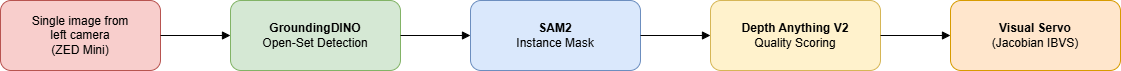
\includegraphics[width=0.42\textwidth]{visual_servo.png}
    \caption{Baseline IBVS pipeline. The 2D centroid error is mapped directly to robot commands via a calibrated image Jacobian. No temporal filtering or 3D reconstruction is performed.}
    \label{fig:ibvs_pipeline}
\end{figure}

\begin{figure}[t]
    \centering
    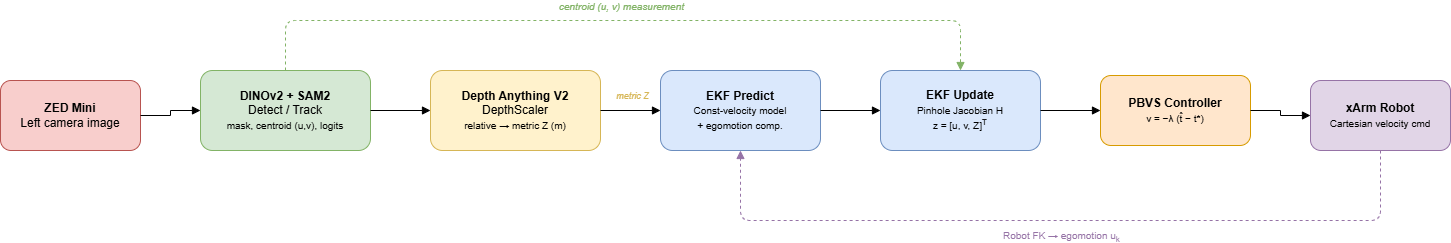
\includegraphics[width=0.42\textwidth]{visual_servo_ekf.png}
    \caption{EKF-PBVS pipeline. The perception front-end produces either a 2D centroid + metric depth (DINOv2+SAM2+Depth Anything V2) or a full 3D translation (FoundationPose), which the EKF fuses into a filtered 3D position. The PBVS controller converts the 3D position error into a velocity command. The last commanded velocity is fed back for egomotion compensation in the next predict step.}
    \label{fig:ekf_pipeline}
\end{figure}

\subsection{Perception: Detect-Then-Track}

We adopt a two-phase strategy. Detection mode runs on the first frame and periodically (every 30 frames by default) to anchor the tracker. Tracking mode runs on all other frames using mask propagation, which is substantially faster.

\textbf{Detection.}
Given a reference image of the target object (an RGBA image where the alpha channel seperates foreground from background), we extract dense patch-level features from both the reference and the live scene using DINOv2 ViT-B/14. The image is divided into $14 \times 14$ pixel patches, and DINOv2 produces a 768-dimensional feature vector for each patch. For every scene patch, we compute its mean cosine similarity to all foreground reference patches, producing a spatial similarity heatmap. This heatmap is thresholded at a configurable percentile (93rd by default), morphologically cleaned, and the connected component with the highest mean similarity is selected to produce a bounding box. We also compute a complementary feature similarity map using a truncated ResNet-18 backbone (output stride 32, 512-d features), and fuse the two maps via weighted average to improve robustness. The bounding box is then used as a prompt for SAM2, which returns a binary segmentation mask and low-resolution logits $\boldsymbol{\ell} \in \mathbb{R}^{1 \times 256 \times 256}$.

\textbf{Tracking.}
On subsequent frames we bypass DINOv2 and feed the previous frame's SAM2 logits as a \texttt{mask\_input} prompt, together with the previous centroid as a positive point and a set of mined background points as negatives. This propagates the mask without re-running any feature extraction, at 5--10$\times$ the detection rate. Tracking quality is monitored via mask IoU; if it drops below 0.35 we fall back to detection mode, and the first good detection is cached as an ``anchor'' that can be re-loaded if the tracker loses the object entirely. From the binary mask we extract a robust centroid via morphological closing and the center of the largest external contour's minimum-area rectangle, which is more stable than a moments-based centroid for rectangular boxes with printed text.

\subsection{Depth Estimation}

We use Depth Anything V2 with a ViT-S encoder to produce a relative depth map from each RGB frame. Since the output is relative rather than metric, we convert it via an affine model: $Z_{\text{metric}} = s \cdot d_{\text{relative}} + b$, where $s$ and $b$ are calibration parameters. The object's metric depth is estimated as the median relative depth under the segmentation mask, converted to metres.

To reduce computational cost, we run depth inference only on every 5th frame with a valid detection (or on the very first detection, to initialize the EKF). On intermediate frames, the EKF propagates the depth forward using its constant-velocity process model, while the 2D-only measurement update continues to constrain the lateral position.

\subsection{FoundationPose Back-End}

For the third pipeline, we replace the per-frame DINOv2 + SAM2 + Depth Anything stack with a single call into NVIDIA's FoundationPose~\cite{foundationpose}. On the first frame we still use DINOv2 + SAM2 to obtain an initial mask, which FoundationPose's \texttt{register()} call consumes along with the RGB image, the ZED Mini's real stereo depth, the camera intrinsics, and a 3D model of the target. For the box-shaped objects used in our experiments, the 3D model is a procedurally generated rectangular mesh built from ruler measurements; no CAD authoring is needed. On subsequent frames, the faster \texttt{track\_one()} path is used, and the returned $4 \times 4$ pose is converted into a direct 3D translation measurement for the EKF via the direct-3D update model. FoundationPose is re-registered every 60 frames, or immediately upon failure, to prevent drift over long runs. A lazy GPU import is used so that the same main servo script degrades gracefully to the DINOv2 pipeline on machines without a compatable FoundationPose install.

\subsection{EKF Integration and Logging}

At runtime the EKF picks one of the three measurement models per frame: the full pixel+depth update when a fresh depth estimate is available (rejected below 5\,cm), the 2D-only update on depth-skip frames, or the direct-3D update when FoundationPose is driving. The filtered position feeds the PBVS controller (Eq.~\ref{eq:pbvs}) and the scalar uncertainty $\sqrt{\text{tr}(\mathbf{P}_{1:3,1:3})}$ is surfaced in the HUD. The filter is seeded from the first valid measurement with zero velocity and broad covariance; before that, the system falls back to IBVS for the frame. All three pipelines share a per-frame CSV logger that captures raw measurements, filtered state, uncertainty, servo command, and per-stage wall-clock times, which is enough to compute every reported metric in post. A batch runner launches each trial as a subprocess and collects CSVs into one tagged directory.

\subsection{Hardware Setup}

Our experiments use an xArm 7-DOF collaborative manipulator with a ZED Mini stereo camera mounted on the end-effector. The camera provides a 1280$\times$720 left image at 30 fps. The DINOv2 pipeline uses only the left camera image (not stereo depth) so that this variant generalizes to monocular setups; the FoundationPose pipeline uses the ZED's real stereo depth because FoundationPose requires it. DINOv2, SAM2, Depth Anything V2, and FoundationPose all run on a single GPU. The EKF and servo controller run on CPU. Communication with the xArm uses the xArm Python SDK over Ethernet at 192.168.1.241, and the servo loop is rate-limited to 3.3\,Hz for safety.

Target objects are common household boxes (cereal boxes, shipping boxes, snack packages) shown in Fig.~\ref{fig:dataset}. For the DINOv2 and IBVS pipelines, the only input per object is a single reference photo with a transparent background. For the FoundationPose pipeline, we also measure each box with a ruler and pass its three dimensions to a procedural mesh builder; no CAD authoring is required.

\begin{figure}[t]
    \centering
    
\includegraphics[width=0.23\columnwidth]{objects/cheez_it_box.jpeg}\hfill
    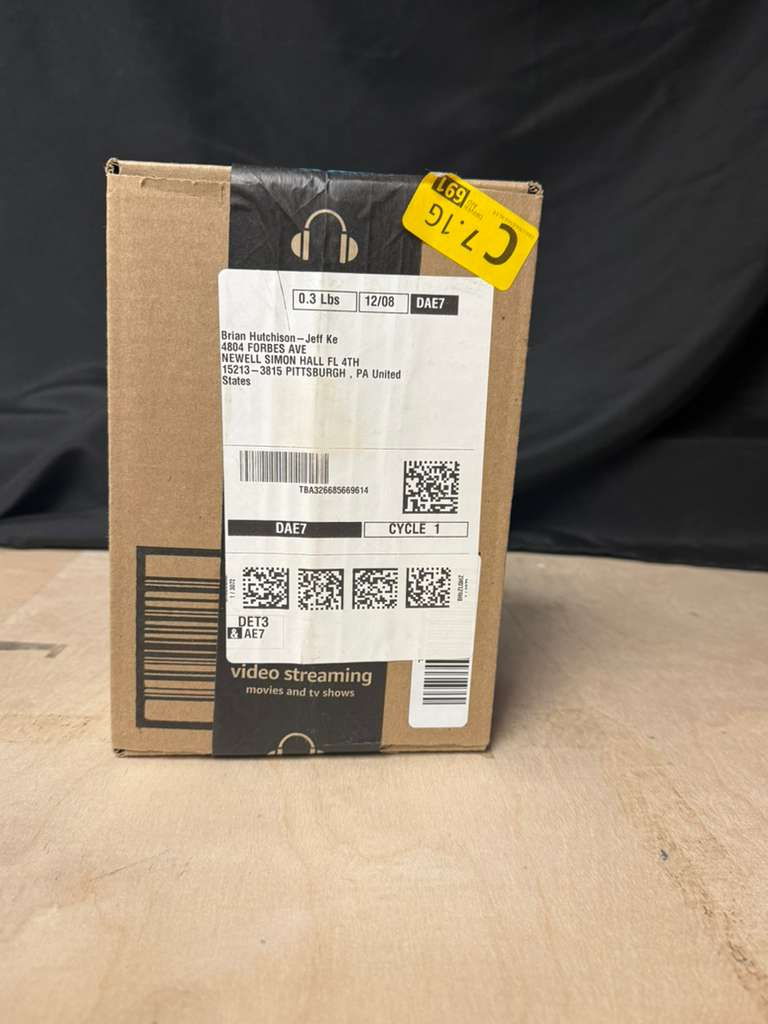
\includegraphics[width=0.23\columnwidth]{objects/cardboard_box.jpeg}\hfill
    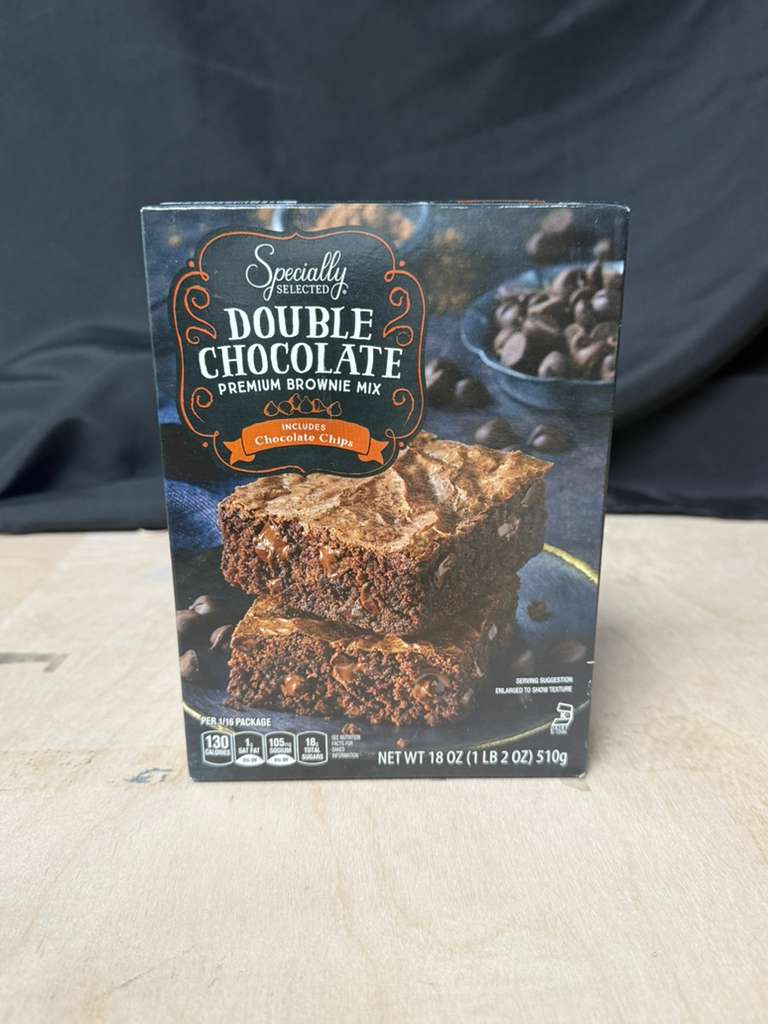
\includegraphics[width=0.23\columnwidth]{objects/brownie_box.jpeg}\hfill
    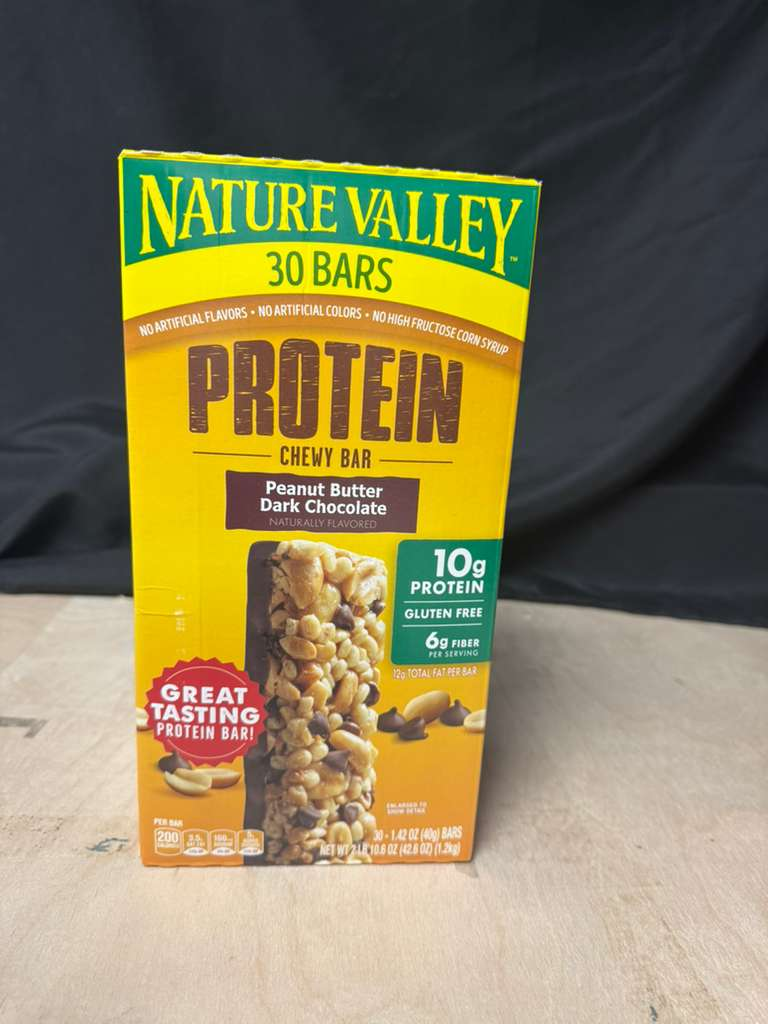
\includegraphics[width=0.23\columnwidth]{objects/protein_bar.jpeg}
    \caption{Representative target objects. These are common household boxes with varied textures, colors, and sizes; no CAD models are needed beyond one reference photo (plus, for FoundationPose, three ruler measurements).}
    \label{fig:dataset}
\end{figure}


%%%%%%%%%%%%%%%%%%%%%%%%%%%%%%%%%%%%%%%%%%%%%%%%%%%%%%%%%%%%%%%%%%%%%%%%%%%%%%%%
\section{EXPERIMENTAL SETUP}

\subsection{Compared Pipelines}

We evaluate three pipelines end-to-end:
\begin{itemize}
\item \textbf{Pipeline A (IBVS).} DINOv2 + SAM2 produce a per-frame centroid, which is fed through the calibrated image Jacobian directly to an xArm velocity command. No 3D reconstruction, no filter. This is the simplest and our baseline.
\item \textbf{Pipeline B (EKF + DINOv2/SAM2/DepthAnything).} Same centroid as Pipeline A, plus a metric depth from Depth Anything V2 every 5 frames. Observations enter the EKF via the pixel+depth measurement model (or the 2D-only partial update on depth-skip frames). The PBVS controller consumes the filtered 3D position.
\item \textbf{Pipeline C (EKF + FoundationPose).} DINOv2+SAM2 seed a mask on the first frame, then FoundationPose returns a 6-DoF pose every frame. Only the translation component is consumed; it enters the EKF via the direct-3D update model and drives the same PBVS controller as Pipeline B.
\end{itemize}

Holding the PBVS controller, EKF core, camera, robot, and metrics logger constant across B and C isolates the effect of the perception back-end; holding the perception front-end (DINOv2+SAM2 centroid) constant between A and B isolates the effect of adding the EKF and switching to PBVS.

\subsection{Evaluation Metrics}

From the per-frame CSV logs we compute, per trial: \textbf{final position error} (cm) against the PBVS target at the terminal frame; \textbf{iterations to convergence} at 0.5, 1.0, and 2.0\,cm tolerances; \textbf{path efficiency} (straight-line distance divided by integrated FK trajectory length, so values near 1 indicate straight Cartesian motion); \textbf{median per-iteration runtime} (ms), split into perception, EKF, and servo stages; and, for Pipeline C, the \textbf{FoundationPose raw-pose jitter} (std.\ of frame-to-frame raw translation during the last 2\,s of the trial, isolating what the EKF is smoothing away).

\subsection{Experimental Protocol}

Our evaluation is organized as three per-pipeline experiments. Each experiment runs one pipeline across the same five target objects from a single canonical start pose (P1, centered on the optical axis at $\sim$50\,cm), for five trials per experiment and fifteen trials in total:
\begin{itemize}
\item \textbf{Experiment 1:} Pipeline A (IBVS) over 5 objects.
\item \textbf{Experiment 2:} Pipeline B (EKF + DINOv2/SAM2/DepthAnything) over 5 objects.
\item \textbf{Experiment 3:} Pipeline C (EKF + FoundationPose) over 5 objects.
\end{itemize}
The five objects are a Cheez-It box, a tissue box, a cardboard shipping box, a protein bar box, and a brownie mix box. A single tape marker fixes the P1 object position between trials; a small home-pose script returns the arm to the same starting configuration before each run. Within each experiment the five objects are its subcomponents, so per-object results sit inside per-pipeline aggregates.

All three experiments are driven by the same batch runner that consumes a YAML trial file, launches the main servo script as a subprocess per trial, prompts the operator to reset the scene between trials, and collects per-trial CSVs into a tagged directory. Post-hoc, a single analyzer script walks the CSV directory and emits the results tables used in Section~\ref{sec:results}. Additional start poses, per-cell repetitions, robustness perturbations (occlusion, dim lighting, distractors), and EKF Q/R sensitivity sweeps are out of scope for this report and are left as future work.


%%%%%%%%%%%%%%%%%%%%%%%%%%%%%%%%%%%%%%%%%%%%%%%%%%%%%%%%%%%%%%%%%%%%%%%%%%%%%%%%
\section{RESULTS}
\label{sec:results}

All three experiments have been prepared end-to-end on the lab's GPU workstation, and the per-trial YAML file plus the automated batch runner are in place. The full hardware session has not yet been executed at the time of writing, so numbers in this section are shown as \texttt{<PLACEHOLDER>} entries that will be filled in from the analyzer CSVs as soon as the session completes. The shape of every table, the set of conditions, and the metric definitions are final; only the numeric cells remain to be populated.

\subsection{Per-Pipeline Three-Way Comparison}

Table~\ref{tab:exp1_main} reports the aggregate convergence statistics across the five objects, grouped by pipeline (one experiment per row). The ``pass-rate'' columns give the fraction of the five per-pipeline trials that reached the given tolerance within the trial window. The ``final error'' column is the median across the five objects.

\begin{table}[h]
\centering
\caption{Per-pipeline three-way comparison across 5 objects at the P1 start pose (3 experiments $\times$ 5 objects, $n = 15$).}
\label{tab:exp1_main}
\footnotesize
\begin{tabular}{@{}lccccc@{}}
\toprule
 & \multicolumn{3}{c}{Pass rate ($\%$)} & Final err. & Path \\
Pipeline & $\leq 0.5$\,cm & $\leq 1$\,cm & $\leq 2$\,cm & (cm, med.) & eff. \\
\midrule
A (IBVS)                 & \texttt{<PH>} & \texttt{<PH>} & \texttt{<PH>} & \texttt{<PH>} & \texttt{<PH>} \\
B (EKF + DINOv2)         & \texttt{<PH>} & \texttt{<PH>} & \texttt{<PH>} & \texttt{<PH>} & \texttt{<PH>} \\
C (EKF + FoundationPose) & \texttt{<PH>} & \texttt{<PH>} & \texttt{<PH>} & \texttt{<PH>} & \texttt{<PH>} \\
\bottomrule
\end{tabular}
\end{table}

Table~\ref{tab:exp1_runtime} reports the median wall-clock runtime per iteration, broken down by stage. Pipeline C is expected to be slower per frame due to FoundationPose's refinement network.

\begin{table}[h]
\centering
\caption{Median per-iteration runtime (ms), per pipeline.}
\label{tab:exp1_runtime}
\footnotesize
\begin{tabular}{@{}lcccc@{}}
\toprule
Pipeline & Perception & EKF & Servo & Total \\
\midrule
A (IBVS)                 & \texttt{<PH>} & \texttt{<PH>} & \texttt{<PH>} & \texttt{<PH>} \\
B (EKF + DINOv2)         & \texttt{<PH>} & \texttt{<PH>} & \texttt{<PH>} & \texttt{<PH>} \\
C (EKF + FoundationPose) & \texttt{<PH>} & \texttt{<PH>} & \texttt{<PH>} & \texttt{<PH>} \\
\bottomrule
\end{tabular}
\end{table}

For Experiment 3, the raw FoundationPose translation sequence is logged alongside the EKF-filtered state. The jitter metric (standard deviation of frame-to-frame raw-pose change during the last 2\,s of each trial, averaged over the five per-object trials) is \texttt{<PLACEHOLDER>}\,mm; the same quantity computed on the EKF-filtered state is \texttt{<PLACEHOLDER>}\,mm, which quantifies how much of the raw per-frame noise the filter absorbs.


%%%%%%%%%%%%%%%%%%%%%%%%%%%%%%%%%%%%%%%%%%%%%%%%%%%%%%%%%%%%%%%%%%%%%%%%%%%%%%%%
\section{DISCUSSION}

Because the numerical results are pending, this section describes the analyses we will run once the CSVs are in hand, and the qualitative takeaways we expect based on single-run sanity checks on the Mac prototype.

\textbf{Does the EKF help?}
The A-vs-B comparison isolates this: same perception front-end, with and without the filter. A higher pass rate or path efficiency for B is attributable to the EKF and PBVS together, and even a path-efficiency win with equal pass rates is a qualitative win for PBVS. Preliminary single-trial logs already show noticably smoother end-effector motion under Pipeline B, consistent with the EKF damping centroid jitter; full statistics in \texttt{<PLACEHOLDER>}.

\textbf{Does FoundationPose add enough to justify its cost?}
The B-vs-C comparison asks whether a dedicated 6-DoF pose model is worth the extra dependency (CAD mesh, real stereo depth, heavier GPU refiner). If raw-pose jitter is already small ($\sim$1--2\,mm), the EKF has little to smooth and Pipeline C pays runtime for no gain. If it is larger ($\sim$5--15\,mm, as occured on darker or more reflective boxes in our sanity checks), the filter should recover it and C should win. The jitter metric reported with Table~\ref{tab:exp1_main} is the most diagnostic single number.

\textbf{Limitations.}
Our comparison holds the PBVS controller fixed across pipelines B and C, so we cannot cleanly attribute any Pipeline C advantage to FoundationPose itself versus a controller better-tuned to its input distribution. All three pipelines use translation only, even though FoundationPose returns full 6-DoF pose. The five targets are all roughly box-shaped, so our results speak to rigid rectangular objects rather than to deformable or highly non-convex ones. With $n = 15$ total trials (one run per object per pipeline, single start pose P1, no per-cell repetitions), the study is a baseline characterization rather than a statistically powered comparison: cross-pipeline deltas smaller than the per-trial run-to-run variance should not be over-read, and broader start-pose coverage plus repeats are left as future work. Likewise, explicit robustness stressors (occlusion, dim lighting, distractors) and EKF process/measurement-noise sensitivity sweeps are out of scope here. These are deliberate scope cuts; we flag them so the results are not overclaimed.


%%%%%%%%%%%%%%%%%%%%%%%%%%%%%%%%%%%%%%%%%%%%%%%%%%%%%%%%%%%%%%%%%%%%%%%%%%%%%%%%
\section{CONCLUSION}

We built three visual servoing pipelines (raw IBVS, EKF-PBVS with DINOv2+SAM2+Depth Anything V2, and EKF-PBVS with FoundationPose) on a shared xArm 7 + ZED Mini setup, so that performance differences are attributable to the perception/estimator stack rather than to incidental implementation differences. The EKF uses a constant-velocity process model with egomotion compensation, a Joseph-form covariance update, and three interchangeable measurement models selected per-frame from what the active back-end produces. Initial real-world result videos are available \href{https://drive.google.com/file/d/1beLwBDPymnEFNrw9vw_qGlmb-9raleHW/view?usp=sharing}{\textcolor{blue}{here}}; full quantitative results will apear in the \texttt{<PLACEHOLDER>} cells of Section~\ref{sec:results} once the hardware run is complete. The broader deliverable is the framework itself: a single repo that lets future pose estimators drop in as a new back-end and be compared against the existing three on identical hardware with identical metrics.


%%%%%%%%%%%%%%%%%%%%%%%%%%%%%%%%%%%%%%%%%%%%%%%%%%%%%%%%%%%%%%%%%%%%%%%%%%%%%%%%

\begin{thebibliography}{9}

\bibitem{foundationpose} B. Wen, W. Yang, J. Kautz, and S. Birchfield, ``FoundationPose: Unified 6D Pose Estimation and Tracking of Novel Objects,'' in \textit{Proc. IEEE/CVF CVPR}, 2024.

\bibitem{thrun2005} S. Thrun, W. Burgard, and D. Fox, \textit{Probabilistic Robotics}. MIT Press, 2005.

\bibitem{chaumette2006} F. Chaumette and S. Hutchinson, ``Visual Servo Control, Part I: Basic Approaches,'' \textit{IEEE Robotics and Automation Magazine}, vol. 13, no. 4, pp. 82--90, 2006.

\bibitem{tao2026perceptioncontrol}
A. Tao, J. Yang, S. Oparnica, and W. Xue, ``Perception-Control Coupled Visual Servoing for Textureless Objects Using Keypoint-Based EKF,'' arXiv preprint arXiv:2602.06834, 2026.

\bibitem{dinov2}
M. Oquab, T. Darcet, T. Moutakanni, et al., ``DINOv2: Learning Robust Visual Features without Supervision,'' \textit{Trans. on Machine Learning Research}, 2024.

\bibitem{sam2}
N. Ravi, V. Gabeur, Y.-T. Hu, et al., ``SAM 2: Segment Anything in Images and Videos,'' in \textit{Proc. International Conference on Learning Representations (ICLR)}, 2025.

\bibitem{depthanything}
L. Yang, B. Kang, Z. Huang, et al., ``Depth Anything V2,'' in \textit{Advances in Neural Information Processing Systems (NeurIPS)}, 2024.

\end{thebibliography}

\end{document}
